\let\negmedspace\undefined
\let\negthickspace\undefined
\documentclass[journal,12pt,onecolumn]{IEEEtran}
\usepackage{cite}
\usepackage{amsmath,amssymb,amsfonts,amsthm}
\usepackage{algorithmic}
\usepackage{graphicx}
\graphicspath{{./figs/}}
\usepackage{textcomp}
\usepackage{xcolor}
\usepackage{txfonts}
\usepackage{listings}
\usepackage{enumitem}
\usepackage{mathtools}
\usepackage{gensymb}
\usepackage{comment}
\usepackage{caption}
\usepackage[breaklinks=true]{hyperref}
\usepackage{tkz-euclide} 
\usepackage{listings}
\usepackage{gvv}                                        
%\def\inputGnumericTable{}                                 
\usepackage[latin1]{inputenc}     
\usepackage{xparse}
\usepackage{color}                                            
\usepackage{array}                                            
\usepackage{longtable}                                       
\usepackage{calc}                                             
\usepackage{multirow}
\usepackage{multicol}
\usepackage{hhline}                                           
\usepackage{ifthen}                                           
\usepackage{lscape}
\usepackage{tabularx}
\usepackage{array}
\usepackage{float}
%\newtheorem{theorem}{Theorem}[section]
%\newtheorem{theorem}{Theorem}[section]
%\newtheorem{problem}{Problem}
%\newtheorem{proposition}{Proposition}[section]
%\newtheorem{lemma}{Lemma}[section]
%\newtheorem{corollary}[theorem]{Corollary}
%\newtheorem{example}{Example}[section]
%\newtheorem{definition}[problem]{Definition}

\begin{document}

\title{4.10.20}
\author{EE25BTECH11018 - Darisy Sreetej}
% \maketitle
% \newpage
% \bigskip
%\begin{document}
{\let\newpage\relax\maketitle}
%\renewcommand{\thefigure}{\theenumi}
%\renewcommand{\thetable}{\theenumi}
\textbf{Question:}\\
Point $\vec{P}(0, 2)$ is the point of intersection of the y-axis and the perpendicular bisector of the line segment joining the points $\vec{A}(-1,1)$ and $\vec{B}(3,3).$\\
\textbf{True} or \textbf{False}\\ 
\solution
\begin{table}[H]
	\centering
	\caption{}
	\begin{tabular}{|c|c|}
\hline
\textbf{Variable} & \textbf{Value} \\
\hline
$A$ & $(0,-\frac{3}{2})$ \\
\hline
$m$ & $\frac{1}{2}$ \\
\hline
\end{tabular}
	\label{}
\end{table}
Let the equation of perpendicular bisector be
\begin{align}
	\vec{n}^\top\vec{x}=C
\end{align}
Let $\vec{R}$ be the midpoint of the line segment $\vec{AB}$
\begin{align}
    \vec{R}=\frac{\vec{A}+\vec{B}}{2} = \frac{\myvec{-1\\1}+\myvec{3\\3}}{2}
\end{align}
\begin{align}
    \vec{R}=\myvec{1\\2}
\end{align}
The direction vector of $\vec{AB}$ is 
\begin{align}
	\vec{n}=\vec{B}-\vec{A}=\myvec{4\\2}
\end{align}
As it passes through the midpoint $\vec{R}$ ,
\begin{align}
\myvec{4&2}\myvec{1\\2}=C
\end{align}
\begin{align}
	C=8
\end{align}
Therefore , the equation of the perpendicular bisector is 
\begin{align}
	\myvec{4\\2}^\top\vec{x}=8
\end{align}
\begin{align}
	\myvec{2\\1}^\top\vec{x}=4
\end{align}
Let $\vec{P}$ be the point of intersection of y-axis with the perpendicular bisector \\
Intersection with y-axis $(x=0)$ ,
\begin{align}
    \myvec{2&1}\myvec{0\\y}=4
\end{align}
\begin{align}
	y=4
\end{align}
Thus,
\begin{align}
	P=\myvec{0\\4}
\end{align}
The point of intersection is $P(0,4)$ \\
Therefore the Statement is \textbf{False}
\begin{figure}[h!]
    \centering
    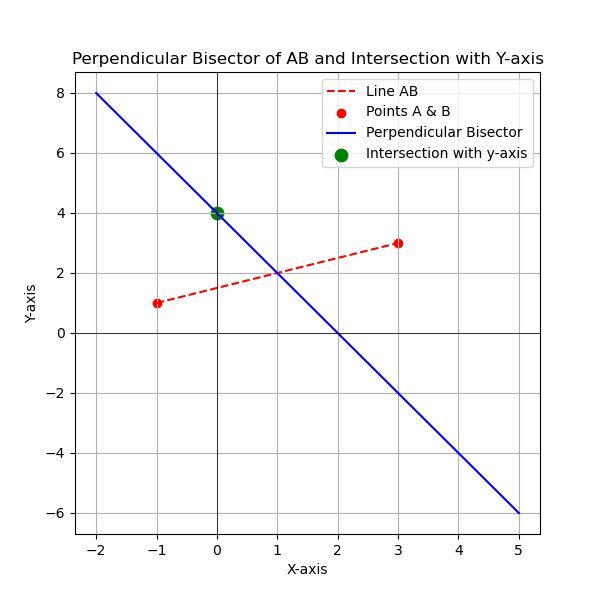
\includegraphics[height=0.5\textheight, keepaspectratio]{figs/fig.png}
    \label{figure_1}
\end{figure}
\end{document}

